% Options for packages loaded elsewhere
\PassOptionsToPackage{unicode}{hyperref}
\PassOptionsToPackage{hyphens}{url}
\PassOptionsToPackage{dvipsnames,svgnames,x11names}{xcolor}
%
\documentclass[
  letterpaper,
  DIV=11,
  numbers=noendperiod]{scrartcl}

\usepackage{amsmath,amssymb}
\usepackage{iftex}
\ifPDFTeX
  \usepackage[T1]{fontenc}
  \usepackage[utf8]{inputenc}
  \usepackage{textcomp} % provide euro and other symbols
\else % if luatex or xetex
  \usepackage{unicode-math}
  \defaultfontfeatures{Scale=MatchLowercase}
  \defaultfontfeatures[\rmfamily]{Ligatures=TeX,Scale=1}
\fi
\usepackage{lmodern}
\ifPDFTeX\else  
    % xetex/luatex font selection
\fi
% Use upquote if available, for straight quotes in verbatim environments
\IfFileExists{upquote.sty}{\usepackage{upquote}}{}
\IfFileExists{microtype.sty}{% use microtype if available
  \usepackage[]{microtype}
  \UseMicrotypeSet[protrusion]{basicmath} % disable protrusion for tt fonts
}{}
\makeatletter
\@ifundefined{KOMAClassName}{% if non-KOMA class
  \IfFileExists{parskip.sty}{%
    \usepackage{parskip}
  }{% else
    \setlength{\parindent}{0pt}
    \setlength{\parskip}{6pt plus 2pt minus 1pt}}
}{% if KOMA class
  \KOMAoptions{parskip=half}}
\makeatother
\usepackage{xcolor}
\setlength{\emergencystretch}{3em} % prevent overfull lines
\setcounter{secnumdepth}{-\maxdimen} % remove section numbering
% Make \paragraph and \subparagraph free-standing
\makeatletter
\ifx\paragraph\undefined\else
  \let\oldparagraph\paragraph
  \renewcommand{\paragraph}{
    \@ifstar
      \xxxParagraphStar
      \xxxParagraphNoStar
  }
  \newcommand{\xxxParagraphStar}[1]{\oldparagraph*{#1}\mbox{}}
  \newcommand{\xxxParagraphNoStar}[1]{\oldparagraph{#1}\mbox{}}
\fi
\ifx\subparagraph\undefined\else
  \let\oldsubparagraph\subparagraph
  \renewcommand{\subparagraph}{
    \@ifstar
      \xxxSubParagraphStar
      \xxxSubParagraphNoStar
  }
  \newcommand{\xxxSubParagraphStar}[1]{\oldsubparagraph*{#1}\mbox{}}
  \newcommand{\xxxSubParagraphNoStar}[1]{\oldsubparagraph{#1}\mbox{}}
\fi
\makeatother

\usepackage{color}
\usepackage{fancyvrb}
\newcommand{\VerbBar}{|}
\newcommand{\VERB}{\Verb[commandchars=\\\{\}]}
\DefineVerbatimEnvironment{Highlighting}{Verbatim}{commandchars=\\\{\}}
% Add ',fontsize=\small' for more characters per line
\usepackage{framed}
\definecolor{shadecolor}{RGB}{241,243,245}
\newenvironment{Shaded}{\begin{snugshade}}{\end{snugshade}}
\newcommand{\AlertTok}[1]{\textcolor[rgb]{0.68,0.00,0.00}{#1}}
\newcommand{\AnnotationTok}[1]{\textcolor[rgb]{0.37,0.37,0.37}{#1}}
\newcommand{\AttributeTok}[1]{\textcolor[rgb]{0.40,0.45,0.13}{#1}}
\newcommand{\BaseNTok}[1]{\textcolor[rgb]{0.68,0.00,0.00}{#1}}
\newcommand{\BuiltInTok}[1]{\textcolor[rgb]{0.00,0.23,0.31}{#1}}
\newcommand{\CharTok}[1]{\textcolor[rgb]{0.13,0.47,0.30}{#1}}
\newcommand{\CommentTok}[1]{\textcolor[rgb]{0.37,0.37,0.37}{#1}}
\newcommand{\CommentVarTok}[1]{\textcolor[rgb]{0.37,0.37,0.37}{\textit{#1}}}
\newcommand{\ConstantTok}[1]{\textcolor[rgb]{0.56,0.35,0.01}{#1}}
\newcommand{\ControlFlowTok}[1]{\textcolor[rgb]{0.00,0.23,0.31}{\textbf{#1}}}
\newcommand{\DataTypeTok}[1]{\textcolor[rgb]{0.68,0.00,0.00}{#1}}
\newcommand{\DecValTok}[1]{\textcolor[rgb]{0.68,0.00,0.00}{#1}}
\newcommand{\DocumentationTok}[1]{\textcolor[rgb]{0.37,0.37,0.37}{\textit{#1}}}
\newcommand{\ErrorTok}[1]{\textcolor[rgb]{0.68,0.00,0.00}{#1}}
\newcommand{\ExtensionTok}[1]{\textcolor[rgb]{0.00,0.23,0.31}{#1}}
\newcommand{\FloatTok}[1]{\textcolor[rgb]{0.68,0.00,0.00}{#1}}
\newcommand{\FunctionTok}[1]{\textcolor[rgb]{0.28,0.35,0.67}{#1}}
\newcommand{\ImportTok}[1]{\textcolor[rgb]{0.00,0.46,0.62}{#1}}
\newcommand{\InformationTok}[1]{\textcolor[rgb]{0.37,0.37,0.37}{#1}}
\newcommand{\KeywordTok}[1]{\textcolor[rgb]{0.00,0.23,0.31}{\textbf{#1}}}
\newcommand{\NormalTok}[1]{\textcolor[rgb]{0.00,0.23,0.31}{#1}}
\newcommand{\OperatorTok}[1]{\textcolor[rgb]{0.37,0.37,0.37}{#1}}
\newcommand{\OtherTok}[1]{\textcolor[rgb]{0.00,0.23,0.31}{#1}}
\newcommand{\PreprocessorTok}[1]{\textcolor[rgb]{0.68,0.00,0.00}{#1}}
\newcommand{\RegionMarkerTok}[1]{\textcolor[rgb]{0.00,0.23,0.31}{#1}}
\newcommand{\SpecialCharTok}[1]{\textcolor[rgb]{0.37,0.37,0.37}{#1}}
\newcommand{\SpecialStringTok}[1]{\textcolor[rgb]{0.13,0.47,0.30}{#1}}
\newcommand{\StringTok}[1]{\textcolor[rgb]{0.13,0.47,0.30}{#1}}
\newcommand{\VariableTok}[1]{\textcolor[rgb]{0.07,0.07,0.07}{#1}}
\newcommand{\VerbatimStringTok}[1]{\textcolor[rgb]{0.13,0.47,0.30}{#1}}
\newcommand{\WarningTok}[1]{\textcolor[rgb]{0.37,0.37,0.37}{\textit{#1}}}

\providecommand{\tightlist}{%
  \setlength{\itemsep}{0pt}\setlength{\parskip}{0pt}}\usepackage{longtable,booktabs,array}
\usepackage{calc} % for calculating minipage widths
% Correct order of tables after \paragraph or \subparagraph
\usepackage{etoolbox}
\makeatletter
\patchcmd\longtable{\par}{\if@noskipsec\mbox{}\fi\par}{}{}
\makeatother
% Allow footnotes in longtable head/foot
\IfFileExists{footnotehyper.sty}{\usepackage{footnotehyper}}{\usepackage{footnote}}
\makesavenoteenv{longtable}
\usepackage{graphicx}
\makeatletter
\def\maxwidth{\ifdim\Gin@nat@width>\linewidth\linewidth\else\Gin@nat@width\fi}
\def\maxheight{\ifdim\Gin@nat@height>\textheight\textheight\else\Gin@nat@height\fi}
\makeatother
% Scale images if necessary, so that they will not overflow the page
% margins by default, and it is still possible to overwrite the defaults
% using explicit options in \includegraphics[width, height, ...]{}
\setkeys{Gin}{width=\maxwidth,height=\maxheight,keepaspectratio}
% Set default figure placement to htbp
\makeatletter
\def\fps@figure{htbp}
\makeatother

\KOMAoption{captions}{tableheading}
\makeatletter
\@ifpackageloaded{caption}{}{\usepackage{caption}}
\AtBeginDocument{%
\ifdefined\contentsname
  \renewcommand*\contentsname{Table of contents}
\else
  \newcommand\contentsname{Table of contents}
\fi
\ifdefined\listfigurename
  \renewcommand*\listfigurename{List of Figures}
\else
  \newcommand\listfigurename{List of Figures}
\fi
\ifdefined\listtablename
  \renewcommand*\listtablename{List of Tables}
\else
  \newcommand\listtablename{List of Tables}
\fi
\ifdefined\figurename
  \renewcommand*\figurename{Figure}
\else
  \newcommand\figurename{Figure}
\fi
\ifdefined\tablename
  \renewcommand*\tablename{Table}
\else
  \newcommand\tablename{Table}
\fi
}
\@ifpackageloaded{float}{}{\usepackage{float}}
\floatstyle{ruled}
\@ifundefined{c@chapter}{\newfloat{codelisting}{h}{lop}}{\newfloat{codelisting}{h}{lop}[chapter]}
\floatname{codelisting}{Listing}
\newcommand*\listoflistings{\listof{codelisting}{List of Listings}}
\makeatother
\makeatletter
\makeatother
\makeatletter
\@ifpackageloaded{caption}{}{\usepackage{caption}}
\@ifpackageloaded{subcaption}{}{\usepackage{subcaption}}
\makeatother

\ifLuaTeX
  \usepackage{selnolig}  % disable illegal ligatures
\fi
\usepackage{bookmark}

\IfFileExists{xurl.sty}{\usepackage{xurl}}{} % add URL line breaks if available
\urlstyle{same} % disable monospaced font for URLs
\hypersetup{
  pdftitle={ALERRT Codebook Template},
  colorlinks=true,
  linkcolor={blue},
  filecolor={Maroon},
  citecolor={Blue},
  urlcolor={Blue},
  pdfcreator={LaTeX via pandoc}}


\title{ALERRT Codebook Template}
\usepackage{etoolbox}
\makeatletter
\providecommand{\subtitle}[1]{% add subtitle to \maketitle
  \apptocmd{\@title}{\par {\large #1 \par}}{}{}
}
\makeatother
\subtitle{v2025}
\author{}
\date{}

\begin{document}
\maketitle

\renewcommand*\contentsname{Table of contents}
{
\hypersetup{linkcolor=}
\setcounter{tocdepth}{3}
\tableofcontents
}

\begin{center}

\includegraphics[width=4.16667in,height=\textheight]{ALERRT Center Badge_Logo PNG.png}
\end{center}

\begin{Shaded}
\begin{Highlighting}[]
\ControlFlowTok{if}\NormalTok{(}\SpecialCharTok{!}\FunctionTok{require}\NormalTok{(tidyverse))\{}
  \FunctionTok{install.packages}\NormalTok{(}\StringTok{"tidyverse"}\NormalTok{, }\AttributeTok{dependencies =} \ConstantTok{TRUE}\NormalTok{)}
  \FunctionTok{library}\NormalTok{(tidyverse)}
\NormalTok{\}}
\CommentTok{\#| warning: false}
\ControlFlowTok{if}\NormalTok{(}\SpecialCharTok{!}\FunctionTok{require}\NormalTok{(rio))\{}
  \FunctionTok{install.packages}\NormalTok{(}\StringTok{"rio"}\NormalTok{, }\AttributeTok{dependencies =} \ConstantTok{TRUE}\NormalTok{)}
  \FunctionTok{library}\NormalTok{(rio)}
\NormalTok{\}}
\CommentTok{\#| warning: false}
\ControlFlowTok{if}\NormalTok{(}\SpecialCharTok{!}\FunctionTok{require}\NormalTok{(summarytools))\{}
  \FunctionTok{install.packages}\NormalTok{(}\StringTok{"summarytools"}\NormalTok{, }\AttributeTok{dependencies =} \ConstantTok{TRUE}\NormalTok{)}
  \FunctionTok{library}\NormalTok{(summarytools)}
\NormalTok{\}}
\end{Highlighting}
\end{Shaded}

\begin{Shaded}
\begin{Highlighting}[]
\NormalTok{create\_codebook }\OtherTok{\textless{}{-}} \ControlFlowTok{function}\NormalTok{(data, }\AttributeTok{magnification =}\NormalTok{ .}\DecValTok{80}\NormalTok{)\{}
\NormalTok{  df }\OtherTok{\textless{}{-}}\NormalTok{ rio}\SpecialCharTok{::}\FunctionTok{import}\NormalTok{(data) }
  \FunctionTok{print}\NormalTok{(}\FunctionTok{dfSummary}\NormalTok{(df, }\AttributeTok{graph.magnif =}\NormalTok{ magnification, }\AttributeTok{valid.col =} \ConstantTok{FALSE}\NormalTok{, }\AttributeTok{na.col =} \ConstantTok{FALSE}\NormalTok{, }\AttributeTok{labels.col =} \ConstantTok{TRUE}\NormalTok{), }\AttributeTok{method =} \StringTok{\textquotesingle{}render\textquotesingle{}}\NormalTok{)}

\NormalTok{\}}

\FunctionTok{create\_codebook}\NormalTok{(}\AttributeTok{data =} \StringTok{"../../../cstat\_bryan\_crime/crime/college\_station\_bryan\_pd\_crimes.xlsx"}\NormalTok{)}
\end{Highlighting}
\end{Shaded}

\begin{longtable}[]{@{}
  >{\centering\arraybackslash}p{(\columnwidth - 8\tabcolsep) * \real{0.2000}}
  >{\raggedright\arraybackslash}p{(\columnwidth - 8\tabcolsep) * \real{0.2000}}
  >{\raggedright\arraybackslash}p{(\columnwidth - 8\tabcolsep) * \real{0.2000}}
  >{\raggedright\arraybackslash}p{(\columnwidth - 8\tabcolsep) * \real{0.2000}}
  >{\raggedright\arraybackslash}p{(\columnwidth - 8\tabcolsep) * \real{0.2000}}@{}}
\toprule\noalign{}
\begin{minipage}[b]{\linewidth}\centering
\textbf{No}
\end{minipage} & \begin{minipage}[b]{\linewidth}\centering
\textbf{Variable}
\end{minipage} & \begin{minipage}[b]{\linewidth}\centering
\textbf{Stats / Values}
\end{minipage} & \begin{minipage}[b]{\linewidth}\centering
\textbf{Freqs (\% of Valid)}
\end{minipage} & \begin{minipage}[b]{\linewidth}\centering
\textbf{Graph}
\end{minipage} \\
\midrule\noalign{}
\endhead
\bottomrule\noalign{}
\endlastfoot
1 & City / Year {[}character{]} &
\begin{minipage}[t]{\linewidth}\raggedright
\begin{longtable}[]{@{}l@{}}
\toprule\noalign{}
\endhead
\bottomrule\noalign{}
\endlastfoot
1. Bryan 2011 \\
2. Bryan 2012 \\
3. Bryan 2013 \\
4. Bryan 2014 \\
5. Bryan 2015 \\
6. Bryan 2016 \\
7. Bryan 2017 \\
8. Bryan 2018 \\
9. Bryan 2019 \\
10. Bryan 2020 \\
{[} 15 others {]} \\
\end{longtable}
\end{minipage} & \begin{minipage}[t]{\linewidth}\raggedright
\begin{longtable}[]{@{}rlrl@{}}
\toprule\noalign{}
\endhead
\bottomrule\noalign{}
\endlastfoot
1 & ( & 4.0\% & ) \\
1 & ( & 4.0\% & ) \\
1 & ( & 4.0\% & ) \\
1 & ( & 4.0\% & ) \\
1 & ( & 4.0\% & ) \\
1 & ( & 4.0\% & ) \\
1 & ( & 4.0\% & ) \\
1 & ( & 4.0\% & ) \\
1 & ( & 4.0\% & ) \\
1 & ( & 4.0\% & ) \\
15 & ( & 60.0\% & ) \\
\end{longtable}
\end{minipage} &
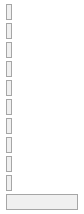
\includegraphics{alerrt_codebook_template_files/mediabag/7GHRIEAAAACdFJOUwAAd.png} \\
2 & Arson {[}numeric{]} & \begin{minipage}[t]{\linewidth}\raggedright
\begin{longtable}[]{@{}l@{}}
\toprule\noalign{}
\endhead
\bottomrule\noalign{}
\endlastfoot
Mean (sd) : 17.4 (9) \\
min ≤ med ≤ max: \\
4 ≤ 16 ≤ 36 \\
IQR (CV) : 9.8 (0.5) \\
\end{longtable}
\end{minipage} & \begin{minipage}[t]{\linewidth}\raggedright
\begin{longtable}[]{@{}rlrlrl@{}}
\toprule\noalign{}
\endhead
\bottomrule\noalign{}
\endlastfoot
4 & : & 1 & ( & 10.0\% & ) \\
9 & : & 1 & ( & 10.0\% & ) \\
11 & : & 1 & ( & 10.0\% & ) \\
15 & : & 1 & ( & 10.0\% & ) \\
16 & : & 2 & ( & 20.0\% & ) \\
21 & : & 1 & ( & 10.0\% & ) \\
22 & : & 1 & ( & 10.0\% & ) \\
24 & : & 1 & ( & 10.0\% & ) \\
36 & : & 1 & ( & 10.0\% & ) \\
\end{longtable}
\end{minipage} &
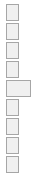
\includegraphics{alerrt_codebook_template_files/mediabag/DEUxUbDfjTsR6IYtvCjJ.png} \\
3 & Sexual\_Assault {[}numeric{]} &
\begin{minipage}[t]{\linewidth}\raggedright
\begin{longtable}[]{@{}l@{}}
\toprule\noalign{}
\endhead
\bottomrule\noalign{}
\endlastfoot
Mean (sd) : 51.8 (21.8) \\
min ≤ med ≤ max: \\
10 ≤ 53 ≤ 116 \\
IQR (CV) : 22 (0.4) \\
\end{longtable}
\end{minipage} & 23 distinct values &
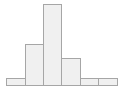
\includegraphics{alerrt_codebook_template_files/mediabag/fYSou8gAAAAAElFTkSuQ.png} \\
4 & Burglary {[}numeric{]} & \begin{minipage}[t]{\linewidth}\raggedright
\begin{longtable}[]{@{}l@{}}
\toprule\noalign{}
\endhead
\bottomrule\noalign{}
\endlastfoot
Mean (sd) : 686.2 (425.3) \\
min ≤ med ≤ max: \\
256 ≤ 511 ≤ 1744 \\
IQR (CV) : 660 (0.6) \\
\end{longtable}
\end{minipage} & 25 distinct values &
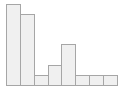
\includegraphics{alerrt_codebook_template_files/mediabag/kZ2ua0WHP6J-3WLXLNSH.png} \\
5 & Robbery {[}numeric{]} & \begin{minipage}[t]{\linewidth}\raggedright
\begin{longtable}[]{@{}l@{}}
\toprule\noalign{}
\endhead
\bottomrule\noalign{}
\endlastfoot
Mean (sd) : 50 (20) \\
min ≤ med ≤ max: \\
19 ≤ 49 ≤ 96 \\
IQR (CV) : 23 (0.4) \\
\end{longtable}
\end{minipage} & 21 distinct values &
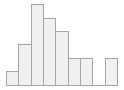
\includegraphics{alerrt_codebook_template_files/mediabag/dwONy5uPnS3t3UPkCPsL.png} \\
6 & Homicide {[}numeric{]} & \begin{minipage}[t]{\linewidth}\raggedright
\begin{longtable}[]{@{}l@{}}
\toprule\noalign{}
\endhead
\bottomrule\noalign{}
\endlastfoot
Mean (sd) : 2.5 (2) \\
min ≤ med ≤ max: \\
0 ≤ 2 ≤ 7 \\
IQR (CV) : 3 (0.8) \\
\end{longtable}
\end{minipage} & \begin{minipage}[t]{\linewidth}\raggedright
\begin{longtable}[]{@{}rlrlrl@{}}
\toprule\noalign{}
\endhead
\bottomrule\noalign{}
\endlastfoot
0 & : & 3 & ( & 12.0\% & ) \\
1 & : & 7 & ( & 28.0\% & ) \\
2 & : & 5 & ( & 20.0\% & ) \\
3 & : & 3 & ( & 12.0\% & ) \\
4 & : & 2 & ( & 8.0\% & ) \\
5 & : & 3 & ( & 12.0\% & ) \\
7 & : & 2 & ( & 8.0\% & ) \\
\end{longtable}
\end{minipage} &
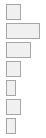
\includegraphics{alerrt_codebook_template_files/mediabag/7GHRIEAAAACdFJOUwAAd1.png} \\
7 & Theft {[}numeric{]} & \begin{minipage}[t]{\linewidth}\raggedright
\begin{longtable}[]{@{}l@{}}
\toprule\noalign{}
\endhead
\bottomrule\noalign{}
\endlastfoot
Mean (sd) : 1650.8 (270) \\
min ≤ med ≤ max: \\
1198 ≤ 1562 ≤ 2137 \\
IQR (CV) : 440 (0.2) \\
\end{longtable}
\end{minipage} & 25 distinct values &
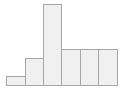
\includegraphics{alerrt_codebook_template_files/mediabag/F0F7mQ-zle7wUgAAAAAS.png} \\
8 & Auto\_Theft {[}numeric{]} &
\begin{minipage}[t]{\linewidth}\raggedright
\begin{longtable}[]{@{}l@{}}
\toprule\noalign{}
\endhead
\bottomrule\noalign{}
\endlastfoot
Mean (sd) : 95 (34.8) \\
min ≤ med ≤ max: \\
36 ≤ 88 ≤ 148 \\
IQR (CV) : 47 (0.4) \\
\end{longtable}
\end{minipage} & 20 distinct values &
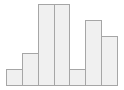
\includegraphics{alerrt_codebook_template_files/mediabag/gHJAAAAABJRU5ErkJggg.png} \\
9 & Aggravated\_Assault {[}numeric{]} &
\begin{minipage}[t]{\linewidth}\raggedright
\begin{longtable}[]{@{}l@{}}
\toprule\noalign{}
\endhead
\bottomrule\noalign{}
\endlastfoot
Mean (sd) : 157.4 (85.4) \\
min ≤ med ≤ max: \\
61 ≤ 127 ≤ 323 \\
IQR (CV) : 139 (0.5) \\
\end{longtable}
\end{minipage} & 23 distinct values &
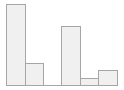
\includegraphics{alerrt_codebook_template_files/mediabag/zEkzebgCpLxcgOsAQCQA.png} \\
\end{longtable}




\end{document}
